\documentclass[conference]{IEEEtran}
\IEEEoverridecommandlockouts
% The preceding line is only needed to identify funding in the first footnote. If that is unneeded, please comment it out.
%\usepackage{cite}
\usepackage{amsmath,amssymb,amsfonts}
\usepackage{amsthm}
\usepackage{algorithmic}
\usepackage{graphicx}
\usepackage{textcomp}
\usepackage{xcolor}
\def\BibTeX{{\rm B\kern-.05em{\sc i\kern-.025em b}\kern-.08em
    T\kern-.1667em\lower.7ex\hbox{E}\kern-.125emX}}
\usepackage{xspace}
\usepackage{hyperref}
\hypersetup{
    colorlinks = true,
    citecolor = {blue}
}

\usepackage[utf8]{inputenc}
\usepackage[T1]{fontenc}
\usepackage{multirow}
\graphicspath{ {images/} }

\usepackage{cleveref}
\usepackage{soul}
\usepackage[
	hyperref=true,
	backref=true,
	bibencoding=utf8,
	backend=biber,
	style=ieee,
	bibstyle=authoryear,
	citestyle=authoryear-comp,
	useprefix=true,
	uniquename=init,
	maxnames=100,
	minnames=3,
	maxcitenames=3,
	mincitenames=1
]{biblatex}
\bibliography{MLE2023}

\RequirePackage{technicalterms}

%%%%% COMMENT SYSTEM %%%%%%%%%%%%%%%%%%%%%%%%
\usepackage{ifthen}
\usepackage{xcolor, color}
\usepackage{comment}
\newboolean{showcomments}
\setboolean{showcomments}{true} % toggle to show or hide comments
\ifthenelse{\boolean{showcomments}} 
{\newcommand{\nb}[2]{
\fcolorbox{gray}{yellow}{\bfseries\sffamily #1}
{$\blacktriangleright$#2$\blacktriangleleft$}
}
\newcommand{\version}{\emph{\scriptsize$-$working$-$}}
}
{\newcommand{\nb}[2]{} 
\newcommand{\version}{}
}
\newcommand\LK[1]{\nb{Lars}{\textcolor{teal}{#1}}}
\newcommand\MA[1]{\nb{Moussa}{\textcolor{blue}{#1}}} 
\newcommand\TW[1]{\nb{Thomas}{\textcolor{red}{#1}}}
\newcommand\HM[1]{\nb{Hossain}{\textcolor{green}{#1}}}
\newcommand\LC[1]{\nb{Loek}{\textcolor{purple}{#1}}}
%%%%%%%%%%%%%%%%%%%%%%%%%%%%%%%%%%%%%%%%

%%%%% PAGE DISPLAY %%%%%%%%%%%%%%%%%%%%%%%%
%%%%% Only for convenience, must be removed
%%%%% for final submission
\pagestyle{plain}
%%%%%%%%%%%%%%%%%%%%%%%%%%%%%%%%%%%%%%%%


\theoremstyle{definition}
\newtheorem{definition}{Definition}[section]

%%%%%%%%%%%%%%%% uml class diagrams %%%%%%%%
\usepackage{pgf-umlcd}
\usepackage{tikzscale}
\usetikzlibrary{calc}
%%%%%%%%%%%%%%%%%%%%%%%%%%%%%%%%%%%%%%%%%%%%
% =================== Configuration of umlcd =======
\renewcommand {\umlfillcolor}{black!0}
\renewcommand {\umltextcolor}{black}
\renewcommand {\umldrawcolor}{black}
% https://tex.stackexchange.com/questions/98021/how-to-extend-pgf-umlcd-with-self-association-connection
\newcommand{\selfassociation}[5]{
\coordinate (a) at ($(#1.north)$);
\coordinate (b) at ($(#1.north) + (0,1)$);
\coordinate (d) at ($(#1.east) + (1,0.8)$);
\coordinate (e) at ($(#1.east) + (0, 0.8)$);
\coordinate (t) at ($(#1.east) + (1,1)$);
\coordinate (c) at ($(d)!(b)!(t)$);
  \draw [umlcd style] (a) -- (b)
  node[midway, left]{#2}
  node[midway, right]{#3};
  \draw [umlcd style] (b) -- (c);
  \draw [umlcd style] (c) -- (d);
  \draw [umlcd style, ->] (d) -- (e)
  node[midway, above]{#4}
  node[midway, below]{#5};
  }
% ====================================================

\begin{document}

\title{Co-Evolving \MetaModels and \ViewTypes\\ in View-Based Development\\
\thanks{This publication is part of the project DIGITAL TWIN (with project number P18-03) of the research programme TTW Perspective which is (partly) financed by the Dutch Research Council (NWO). This work was supported by funding from the topic Engineering Secure Systems of the Helmholtz Association (HGF) and by KASTEL Security Research Labs.}
}


\author{
\IEEEauthorblockN{Lars König}
\IEEEauthorblockA{\textit{KASTEL - Institute of Information }\\
\textit{Security and Dependability}\\
\textit{Karlsruhe Institute of Technology (KIT)}\\
Karlsruhe, Germany \\
\texttt{lars.koenig@kit.edu}\\https://orcid.org/0000-0002-1751-1291}
\and
\IEEEauthorblockN{Thomas Weber}
\IEEEauthorblockA{\textit{KASTEL - Institute of Information }\\
\textit{Security and Dependability}\\
\textit{Karlsruhe Institute of Technology (KIT)}\\
Karlsruhe, Germany \\
\texttt{thomas.weber@kit.edu}\\
https://orcid.org/0009-0001-5775-2225}
\and
\IEEEauthorblockN{Moussa Amrani}
\IEEEauthorblockA{\textit{Faculty of Computer Science}\\
\textit{Namur Digital Institute (NaDI)} \\
\textit{University of Namur}\\
Namur, Belgium \\
\texttt{Moussa.Amrani@unamur.be}\\https://orcid.org/0000-0002-6987-1037}
\and
\IEEEauthorblockN{Hossain Muhammad Muctadir}
\IEEEauthorblockA{\textit{Department of Mathematics and Computer Science} \\
\textit{Eindhoven University of Technology (TU/e)}\\
Eindhoven, The Netherlands \\
\texttt{h.m.muctadir@tue.nl}\\https://orcid.org/0000-0002-2090-4766}
\and
\IEEEauthorblockN{Loek Cleophas}
\IEEEauthorblockA{\textit{Department of Mathematics and Computer Science} \\
\textit{Eindhoven University of Technology (TU/e)}\\
Eindhoven, The Netherlands \\
\texttt{l.g.w.a.cleophas@tue.nl}\\https://orcid.org/0000-0002-7221-3676}
}
\maketitle

\begin{abstract}
View-based development is a successful approach for the development of complex cyber-physical systems.
It uses views to abstract from the complexity of the system and allows the developers to focus on exactly the necessary information for a certain task.
With projective views, the information shown is derived from underlying models, and changes made to the views are reflected back to the models.
Similar to how models conform to a \metamodel, views conform to a \viewtype, which describes what and how the information is presented.
When the underlying \metamodels need to evolve, e.g., due to new requirements, so do the \viewtypes that rely on them.

In this work, we investigate how to assist the \metamodel/view-type co-evolution process by providing suggestions for adapting a \viewtype after a \metamodel change.
To this end, we precisely describe what a suggestion in this context is, and present a list of domain-independent suggestions for the most representative \metamodel evolution steps. 

\sout{We describe how to specialize our approach with domain-specific suggestions, and sketch how a tool based on our approach could be implemented---using recently developed techniques for detecting semantically meaningful \metamodel evolution steps.}
\MA{Careful that the promise of this last sentence is not in the paper!}\HM{I agree. This whole paragraph might go?}

%\TW{\begin{quote}
%    Specifically, in its 2023 edition, the workshop aims to shed light on the strong links between model evolution and sustainability, and in a broader sense, to shed light on the potential of model-centered techniques to drive sustainability initiatives.
%\end{quote} Probably we can say a sentence or two in that direction}
%\LC{Discussed today during call. Seemed to have agreement it's a bit far-fetched, at least, to be more specific than the general 'support for models and model evolution helps for sustainability' claim, and putting a sentence or two in doesn't help for acceptance.}
\end{abstract}

\begin{IEEEkeywords}
View-Based Modelling,
Co-Evolution
\end{IEEEkeywords}

\section{Introduction}
\label{sec:Introduction}

Today's software systems, and systems in general, have reached a complexity which
makes it nearly impossible to comprehend the entire system at once.
This is especially the case when, e.g., in the development of Cyber-Physical Systems,
developers from multiple domains are working together on the same system.
Modern Model-Driven Engineering tools therefore need to provide abstractions of the modeled system.
In order to reduce the accidental complexity for a specific task, tools should present only the necessary part of the system in the most appropriate way.
An established solution for this are \emph{views}, which show a part of the system from a certain \emph{viewpoint} \cite{atkinson_orthographic_2010}.
In a model-driven context, views are usually also models, and therefore conform to a \metamodel,
called a \emph{\viewtype} \cite{goldschmidt_towards_2012}, which specifies 
the information shown in a view and how it is presented.

While for established, general purpose (modeling) languages (e.g., Java, UML, SysML, Simulink), evolution is typically infrequent, for Domain-Specific Languages developed in-house in industrial settings, this may not be the case: there, evolution will typically be more frequent as languages are developed and adapted over time, with increasing insight or to reflect increasing use and capabilities.
Since languages evolve, so do their \metamodels. This is well-known from the literature and industrial practice \cite{durisic_evolution_2014}. Yet as a result of this, \viewtypes depending on such languages and \metamodels need to evolve along with the evolution of the underlying \metamodels. Regardless of the frequency of \metamodel evolution, any view-based framework should support such evolution and hence \metamodel/\viewtype co-evolution, in order for the various views to stay consistent with the models. 

In this paper, we focus on such \metamodel/\viewtype co-evolution which as far as we know has not been considered in the literature before---unlike co-evolution of concrete models (views) with changes in their \metamodel (\viewtype)---known as \metamodel/model co-evolution.
%\LC{You are probably right. I was thinking about \metamodel-model co-evolution, and viewtypes as metamodels}\LK{Is co-evolution of view types and views researched? I would have thought it would be enough to change the view type and re-generate the views with the new view type.}
We focus our attention on \metamodel/\viewtype co-evolution where first the \metamodel is changed, then the \viewtype, since the latter is conceptually typically a \metamodel derived from the former. % (via operations such as filtering, selection, and others). \LK{Should we still mentioned concrete operators? I'm not sure we're actually using them anymore.}
We do not consider scenarios where a \viewtype depends on multiple \metamodels, although our approach remains applicable by merging the required \metamodels into one. %as multiple \metamodels can be integrated into one. \LK{Suggestion: ``[...] although our approach remains applicable by merging the required \metamodels into one.'', since merging multiple \metamodels comes with certain drawbacks.}
%That is, we do not consider evolution scenarios where first the \viewtype is changed and then the underlying \metamodel should be co-evolved; we consider that while conceptually evolution may initially be considered at the \viewtype level, it makes more sense to then consider what needs to change at the \metamodel level to accommodate this, before considering what changes this might trigger on the \viewtype level. 

We offer an approach for co-evolving \viewtypes based on \metamodel changes, in which the so-called \textit{methodologist} \cite{atkinson_orthographic_2010}, i.e.~the language engineer responsible for the \viewtype, is supported by offering them recommendations and considerations to take into account, given specific \metamodel changes and the \viewtype changes that these might require. We emphasize that our approach is a manual one --- given the breadth of potential \metamodel changes and \viewtypes-\metamodel dependencies (directly, or through view generation transformations), it is impossible to determine, without human input, what changes, if any, need to be made to a \viewtype.

Our approach is a generic one, offering domain-independent suggestions for the most important \metamodel evolution steps. Whether and how it is possible and makes sense to also consider domain-specific suggestions for specific application domains or implementation language domains, is a topic for future research. \LC{I've rewritten the preceding to deflect specialization of suggestions to future work; what do you think?}

Our work offers:\LC{thoughts on this welcome}
\begin{itemize}
    \item an approach to offer domain-independent suggestions for the most important \metamodel evolution steps;
    \item the application of such suggestions to an example domain, namely that of \metamodels and \viewtypes for finite state machines;
    \item and a conceptual model for the \viewtype co-evolution suggestions offered by our approach.
%    \item \sout{A means of extending this approach to specific application domains, 
%		as well as implementation language domains.} 
%    \item \sout{The application of the former to the domains of \LC{TODO: once domains settled}, leading to a concrete, partially generic and partially domain-specific lists of suggestions per \metamodel evolution step.}
\end{itemize}
\MA{I would list the following: 
(i) an \emph{approach} and a \emph{conceptual model} for VT/MM co-evolution; 
(ii) a \emph{catalog} [maybe another word?] of suggestions for the key [or ``most important'' as already phrased] evolution
operators; 
(iii) an \emph{illustration} on a simple, yet representative example [without naming it]}

The paper starts by covering background information on view-based development and
\metamodel evolution in \cref{sec:Background}. \cref{sec:Example} describes
a typical scenario for \metamodel/\viewtype co-evolution on a simple example. Then, \cref{sec:Suggestion} explains how \viewtype suggestions are structured, given
change operators on a \metamodel under evolution; these suggestions are then discussed in detail in \cref{sec:Approach}. We present Related Work in \cref{sec:RW}, and discuss strengths and limitations of our approach in \cref{sec:Discussion} before concluding in \cref{sec:Conclusion}.
\section{Background}
\label{sec:Background}

In this section, we will explain the necessary concepts on which our approach builds. First, in \cref{sec:ViewBasedDevelopment}, we will explain different solution strategies to view-based development, as well as a short introduction to the development process in view-based environments. \Cref{sec:ViewGeneration} will then explain how views are generated and the impact of different view generation languages on our approach to \metamodel \viewtype co-evolution. Finally, in \cref{sec:MetaModelEvolution}, we will provide an explanation on how we break down \metamodel evolution in semantically meaningful steps and how these steps can be detected a posteriori.

% \MA{Does it make sense to split the Section into two: (i) Views; (ii) View Generation (or something similar)}

\subsection{View-Based Development}
\label{sec:ViewBasedDevelopment}

There is a distinction between \emph{synthetic} and \emph{projective} approaches to view-based modeling \autocite{atkinson_fundamental_2015}.
In synthetic approaches, the system is represented by the union of all views.
For that purpose, changes must be propagate between the views to ensure the system description is consistent.
This is different in projective approaches where, in addition to the views, an underlying model of the system exists, which is the source of all information.
Views in projective approaches are transient, i.e., not persistent, and generated dynamically from the underlying model whenever they are required \autocite{atkinson_orthographic_2010}.
With projective views, the user is only allowed to interact with the system through the views, while the underlying model is usually hidden.
In particular, when a user wants to make changes to the system, the changes need to be applied to (editable) views first and are then propagated to the underlying model.
The relationship between views, \viewtypes, models and \metamodels in projective approaches is shown in \cref{fig:view_concept}.
The \cite{ISO42010} standard also contains a definition of the \emph{view} concept, as well as of synthetic and projective approaches, but in a broader sense for software architecture and software architecture description languages.

\begin{figure}
    % TODO recreate figure (with \metamodel and \viewtype)
    \begin{center}
        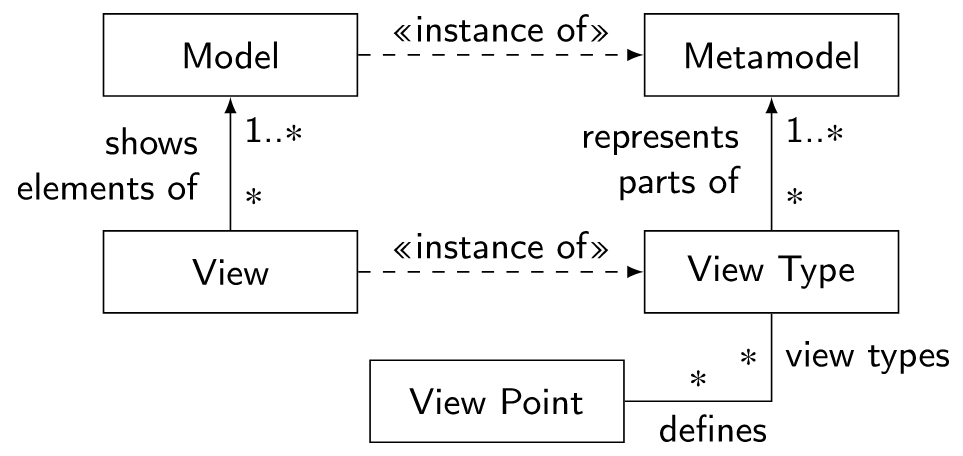
\includegraphics[width=\linewidth]{images/ViewTypeTerminology.png}
    \end{center}

    \caption{Visualization of the view terminology for projective approaches as defined by \textcite{burger_flexible_2014} and \textcite{klare_enabling_2021}.}
    \label{fig:view_concept}
\end{figure}

For projective view-based environments there are different ways of constructing the (single) underlying model (SUM).
\Textcite{atkinson_fundamental_2015} differentiate between \emph{essential} and \emph{pragmatic} SUMs.
With an essential SUM there is a single model, which contains the complete system description and is free of any internal redundancies.
For the synchronization between the views, this is the easiest solution, because the views are simply required to write the changes back to the SUM.
Subsequently generated views are then automatically consistent.
An example of an approach employing an essential SUM is OSM by \textcite{atkinson_orthographic_2010}.
In contrast to a single redundancy-free model, there are also pragmatic approaches where the underlying model consists of multiple submodels.
The main benefit of pragmatic approaches is the construction of the underlying model.
While it is difficult to create a single redundancy-free \metamodel, especially for a domain-spanning system, pragmatic SUMs allow the integration of already available \metamodels, e.g., from development tools used in the various domains.
Additional effort is, however, necessary to keep the models consistent.
One framework for constructing pragmatic SUMs, here called virtual SUMs (V-SUMs), is Vitruvius \autocite{klare_enabling_2021}.

\Textcite{atkinson_orthographic_2010} identified two roles when employing a view-based development process.
First, the \emph{methodologist} is responsible for creating the view-based environment.
For this, the methodologist creates or assembles the SUM, which includes specifying the consistency relations between the models, if necessary.
In addition, they define the view types on the system, including rules how changes are propagated back to the underlying model.
The second role, the \emph{developer}, uses the environment created by the methodologist to develop the actual system.
The developer creates views on the system to inspect its properties and performs changes on them, which are then applied to the underlying model.

\subsection{View Generation}
\label{sec:ViewGeneration}

Since the content of projective views is derived from the underlying model, the methodologist must define a \emph{view generation transformation (VGT)} for each view type, which dynamically creates a view from the model instances when required \autocite{tunjic_synchronization_2015}.
For pragmatic SUMs, the VGTs must be able to combine models from multiple \metamodels, since the content of a view can be scattered over different internal \metamodels \autocite{burger_flexible_2014}.
For users to make changes to the system, views in general must be editable, which requires at least partially bidirectional VGTs.
This may either be achieved by having a transformation language that can derive the reverse direction from the specification of the view generation transformation or by manually writing the transformations for both directions, i.e., the view generation transformation and the transformation of the changes on the view to changes on the models, on which the view is based.
% \MA{The term "bidirectional" assumes that you only define one direction, and the Trafo Framework automatically infers the other direction. This is usually too much trouble: having a spec of both sense can do the trick.}
Of course, there might be cases in which the backpropagation of changes is not possible, e.g., when showing a sum of multiple values, which causes the affected elements to be read-only in the view.
In some cases, the methodologist might restrict the editing capabilities further, e.g., when the view is intended for a specific task where only some of the elements should be edited in the process.
For the definition of the VGTs, common model transformation languages, such as \cite{omg_qvt} or \cite{eclipse_atl}, can be used, as well as formal bidirectional model transformation frameworks, such as the \emph{lenses} framework \autocite{foster_combinators_2007}.
A different approach for the definition of VGTs is \emph{ModelJoin} \autocite{burger_model-join_2016}, which is an operator-based model query language.
ModelJoin also supports the derivation of a view type based on a query.

% TODO may need further justification, also we might not need to focus on a specific model query language if we only differentiate between "included in VT" and "included in VGT"
In our work, we assume that a model query language similar to ModelJoin is used to define the VGTs, since we require semantic information on how a model element is used in a view type.
Our approach will derive this information from the query language operators in which model elements are used in a VGT.
The operators, which we assume to be used in model query languages for view generation, are shown in \cref{fig:model-query-operators}.

\begin{figure}[h]
    \begin{itemize}
        \item \texttt{Select}
        \item \texttt{Filter}
        \item \texttt{Join}
        \item \texttt{Aggregate}
        \item \texttt{Calculate}
    \end{itemize}

    \caption{Proposed set of operators for a model query language for view generation based on \textcite{burger_model-join_2016}.}
    \label{fig:model-query-operators}
\end{figure}

The expected behavior of the model query operators in \cref{fig:model-query-operators} is as follows.
The \texttt{select} operator selects \metamodel elements, which will appear in the view type, while the \texttt{filter} operator is used to define criteria by which model instances are included in a view when generating it.
\MA{So, if I understand correctly, a "select" is a "filter" with no filtering criterium?}
\LK{Not directly. Comparing it to databases, the "select" operator would create the column headers, i.e. specify what kind of data will be presented, while the "filter" operator would define (e.g., by defining a predicate function) which rows from the database will be included in the result. Is this understandable from what I wrote or do you have an idea how I could improve the explanation?}
For the multi-\metamodel case, the \texttt{join} operator connects model instances from different \metamodels.
Both, the \texttt{aggregate} and the \texttt{calculate} operator create new model elements.
While the former combines the values of a single property in multiple instances of a \metaclass, the latter is used to calculate a new property based on multiple existing ones.
Following \textcite{burger_model-join_2016}, we assume this is a reasonable set of operators for the definition of generic views.
\MA{I would have expected a short discussion on OCL beyond the obvious limitation (of handling only one MM).}

\subsection{\Metamodel Evolution}
\label{sec:MetaModelEvolution}

\begin{itemize}
    \item model deltas, atomic changes
    \item catalogue paper
    \item detecting complex changes paper
\end{itemize}

\section{Example Scenario}
\label{sec:Example}

\begin{figure*}
    \centering
    \begin{subfigure}[b]{0.45\textwidth}
			\centering
      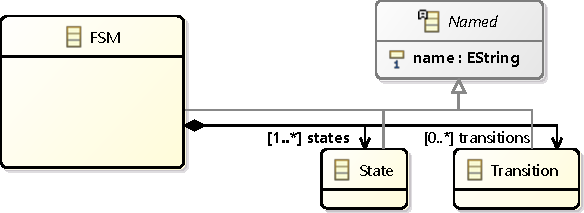
\includegraphics[width=\textwidth]{FSM0.pdf}
      \caption{Initial \metamodel.}
      \label{fig:FSM:Init}
    \end{subfigure}
    \hfill
    \begin{subfigure}[b]{0.45\textwidth}
			\centering
      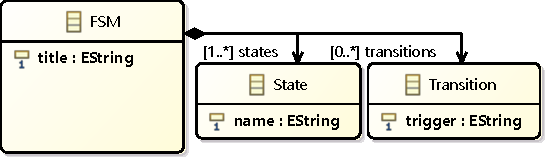
\includegraphics[width=\textwidth]{FSM1.pdf}
      \caption{\textbf{Step 1:} Specifying relevant \textsf{name}s}
      \label{fig:FSM:Relevant}
    \end{subfigure}
    \hfill
    \begin{subfigure}[b]{0.45\textwidth}
			\centering
      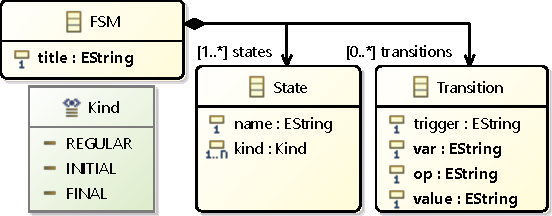
\includegraphics[width=\textwidth]{FSM2.pdf}
      \caption{\textbf{Step 2:} Adding rudimentary guards and \textsf{FINAL}.}
      \label{fig:FSM:Guard}
    \end{subfigure}
    \hfill 
		\begin{subfigure}[b]{0.45\textwidth}
			\centering
      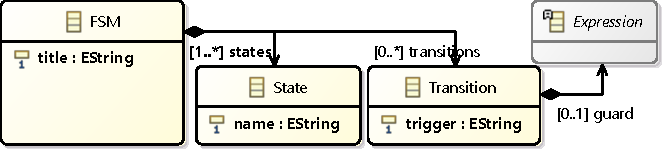
\includegraphics[width=\textwidth]{FSM3.pdf}
      \caption{\textbf{Step 3:} Specifying a fully-fledged \textsf{Expression} for \textsf{guard}s.}
      \label{fig:FSM:Expression}
    \end{subfigure}
    \caption{Three evolution steps for the \textsf{FSM} \metamodel. Note that details, such as the state kind, are omitted in subfigure b.}%\LC{Well, they aren't part of that MM yet, right? State kind only gets introduced in Step 2 so Subfigure c, right?}\LK{But they are already in subfigure a and the text mentions that some details are omitted in subfigure b.}}
    \label{fig:FSM}
\end{figure*}

This Section describes a small, yet representative example of \metamodel
evolution steps on a popular \textsc{Dsl}, the Finite State Machine (\textsf{FSM}).
Note that we simplify the \metamodels and corresponding \viewtypes, to focus 
the discussion only on the parts relevant to co-evolution. 

A methodologist starts with the simple version depicted in \cref{fig:FSM:Init}:
an \textsf{FSM} consists of \textsf{State}s and \textsf{Transition}s. Each class
inherits a \textsf{name} that denotes the \textsf{FSM}'s title, the \textsf{State}'s
name, and the \textsf{Transition}'s trigger. Moreover, \textsf{INITIAL} \textsf{State}s
are distinguished from \textsf{REGULAR} ones to indicate where computations start.
From this initial version, the methodologist defines a \viewtype \textsf{VT\_FSM}
that has two characteristics (cf. \cref{fig:VT}). First, it captures \textsf{Transition}s \emph{inside},
or as part of, \textsf{State}s, to help compute e.g. the set of outgoing 
\textsf{Transition}s from a given \textsf{State}. Second, it represents the various
\textsf{kind}s of \textsf{State}s as a hierarchy, instead of an enumeration,
in order to facilitate the specification of a future visual concrete syntax where
each class is associated to a specific icon.
Additionally, \textsf{VT\_FSM} explicitly computes \textsf{nbStates} and 
\textsf{nbTransitions}, the number of \textsf{State}s and \textsf{Transition}s 
in any given \textsf{FSM} conformant model. A \emph{textual} concrete syntax 
provides a view, conformant to \textsf{VT\_FSM}, of a \textsf{Simple FSM} containing
four \textsf{State}s and six \textsf{Transition}s.


In a first evolution step, the methodologist refines the \textsf{FSM} metamodel,
after noticing that the inherited \textsf{name}s actually play different roles,
by  \emph{pushing down} the \textsf{name} attribute and \emph{renaming} it where
appropriate (other irrelevant details are omitted from \cref{fig:FSM:Relevant}). 
This evolution step does not impact the \viewtypes, but rather the way information
in views is computed: for example, the \textsf{name} of a \textsf{Transition} in
\textsf{VT\_FSM} can no longer be computer using \texttt{t.name} (where 
$\mathsf{t : FSM::Transition}$), but rather with \texttt{t.\textbf{trigger}}. 
The methodologist can take this further by reflecting the \textsf{name}s update
into \textsf{VT\_FSM} to avoid further confusion and keep a direct link with
\textsf{FSM}'s meta-elements.

In a second evolution step, the methodologist wants to extend \textsf{FSM}'s 
behaviour in two ways, leading to the version depicted in \cref{fig:FSM:Guard}. First, by adding \textsf{FINAL} \textsf{State}s,
resulting in \emph{creating} the enumeration literal \textsf{FINAL}.
Second, by adding a rudimentary representation for guards that may prevent 
triggering a \textsf{Transition} when its guard evaluates to \texttt{false}. 
For this purpose, three new attributes are \emph{created} in \textsf{Transition}, allowing to capture
simple expressions over \textsf{var}iables, using boolean and numeric \textsf{value}s
(e.g., \textsf{v = 10} or \textsf{k or l}). After this step, \textsf{VT\_FSM}'s
models may still be valid w.r.t.~the evolved \metamodel (assuming the lack of 
guard is interpreted as a trivial \textsf{true} guard),
but \viewtypes likely have to reflect this new information by \emph{ADD}ing new 
entities in appropriate places (extending the class hierarchy
with a new subclass \textsf{Final}; and adding new attributes for representing 
expressions).

In a final evolution step, the methodologist, confident with the implemented
execution engine, specifies a fully-fledged \textsf{Expression} model,
allowing a \textsf{Transition} to possess a \textsf{guard}, thus \emph{deleting}
the extra attributes added in the previous step. \cref{fig:FSM:Expression} depicts
the resulting \metamodel. Here again, \textsf{VT\_FSM} would likely have to 
choose which information in an \emph{Expression} need to be reflected.
\LK{How does this relate to the view type?}\MA{Added more info: since again, we 
never had a proper example other than just reflecting the MM, we cannot say much here.}

% \HM{I think it might be useful to mention the operators from Table \cref{tab:suggestions} applied to the MM at each step and later connect this with the suggestions?}

\begin{figure}
    \centering
    \begin{subfigure}[b]{\columnwidth}
			\centering
      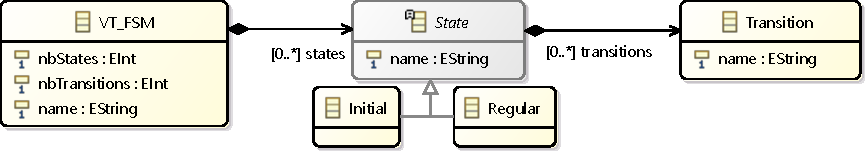
\includegraphics[width=\columnwidth]{FSM_VT.pdf}
      \caption{A \viewtype for \textsf{FSM}, with \textsf{Transition} \emph{inside} \textsf{State}s.
			\LC{Similar comment to LK's on Figure 2 caption: Final subclass of State should be added?}
			\MA{This \viewtype is supposed to be associated with the initial MM. Its 
			co-evolutions are only described in the text, not represented. Again, since the example is cosmetic and only mimic the MM, we cannot say much more!}}
      \label{fig:VT:VMM}
    \end{subfigure}
    \hfill
    \begin{subfigure}[b]{\columnwidth}
			\centering
      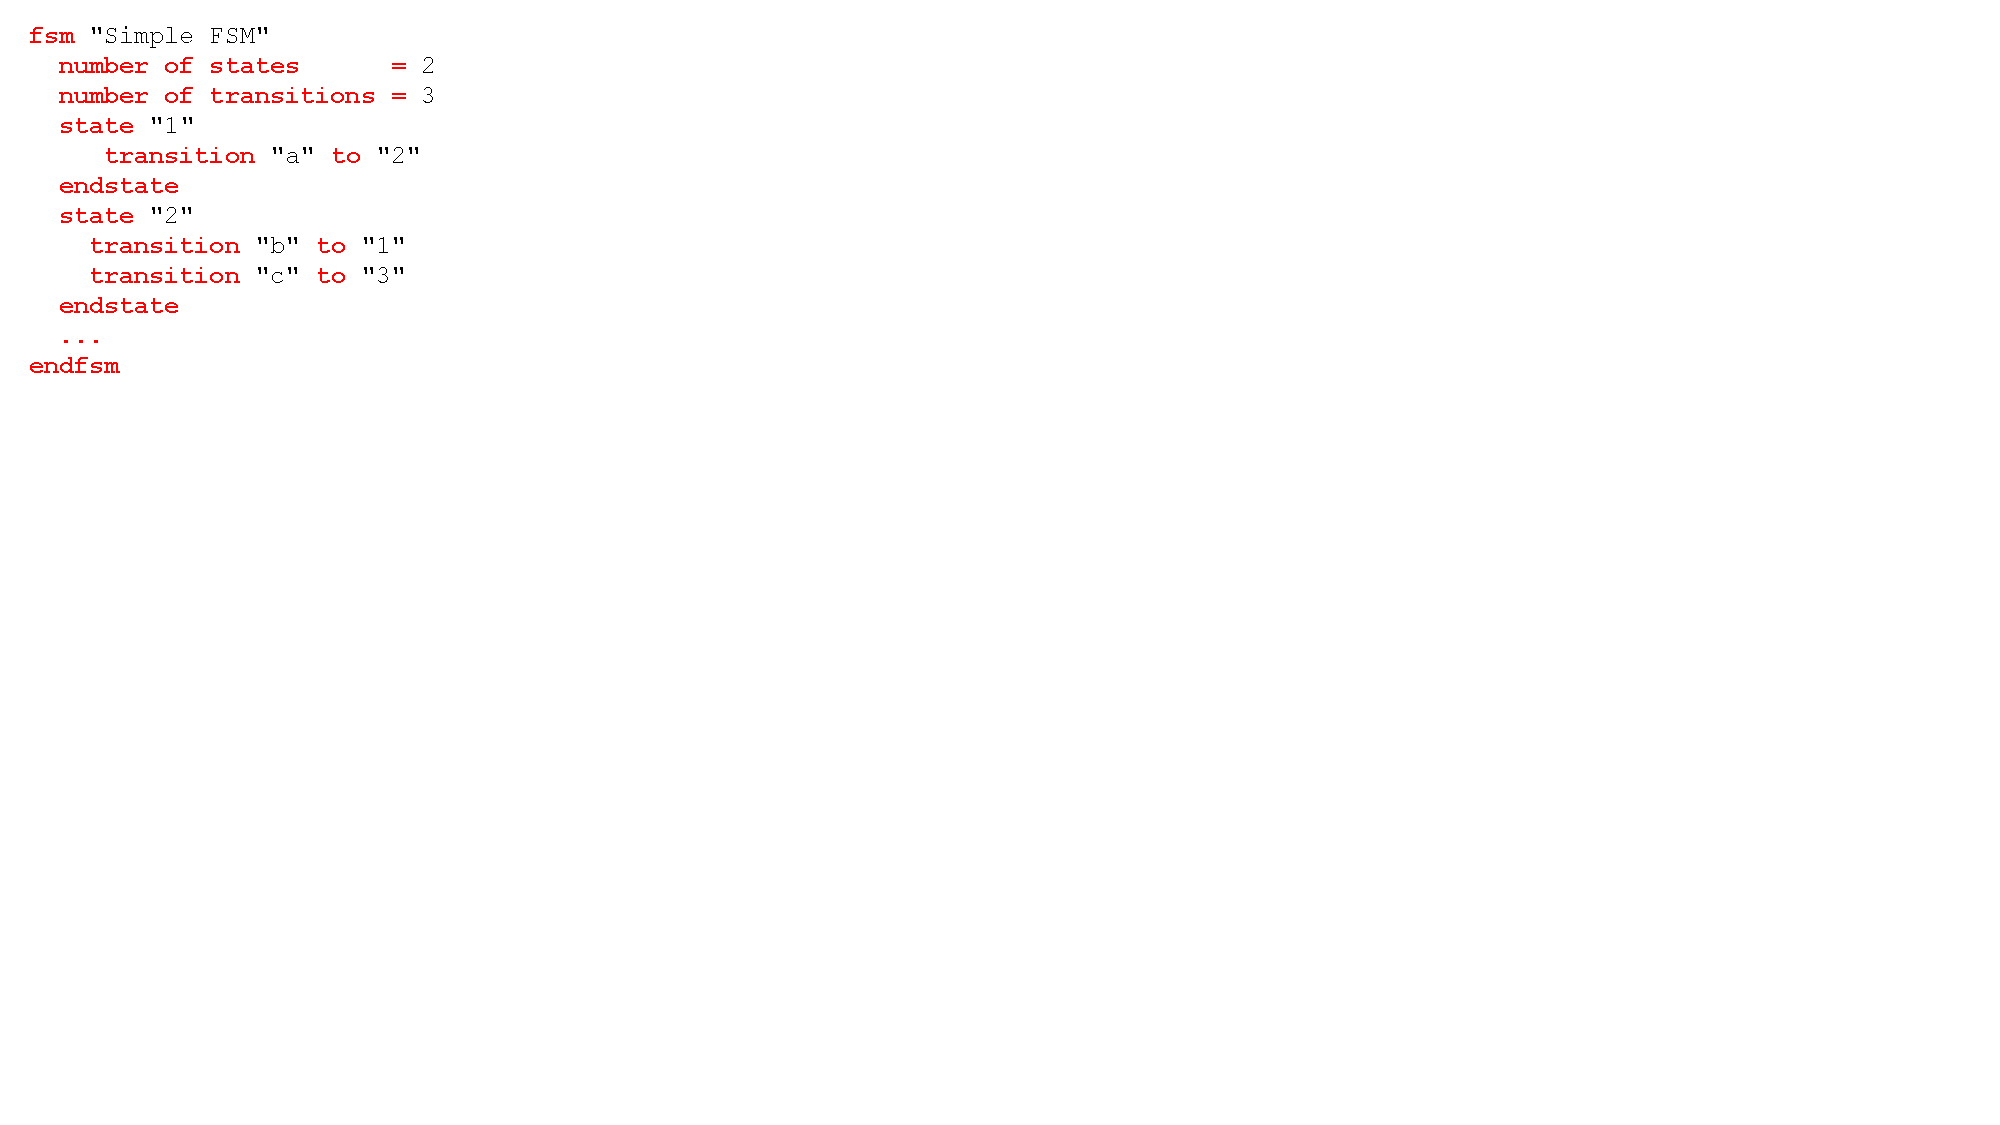
\includegraphics[width=0.5\textwidth, page=1, clip, trim=0cm 12cm 26cm 0cm]{VT.pdf}
      \caption{A textual view of an \textsf{FSM} model named \textsf{Simple FSM} with 4 \textsf{States} and 6 \textsf{Transitions} (details omitted).}
      \label{fig:VT:TM}
    \end{subfigure}
    \caption{A \Viewtype, and an associated view for the \textsf{Simple FSM} model.}
    \label{fig:VT}
\end{figure}

\section{Suggesting Changes In View(s Types)}
\label{sec:Suggestion}

Figure \ref{fig:Suggestion} depicts a \metamodel that capture the
required elements for helping methodologists improve their designs.
On the following, we assume that a methodologist is working on a \metamodel
under evolution \textsf{MM}, that is linked to a family $\mathsf{VT}$ of viewtypes
(i.e. $\mathsf{VT} = (\mathsf{VT}_i)_{i\in [1..n]}$). Note that in the discussion above, when we discuss
\textsf{MM}'s (meta-)elements, we consider \textsf{MM} as a \emph{model}
conforming to a particular meta-\metamodel (such as \textsc{Mof} \cite{TR:OMG-MOF:2016}):
we therefore discuss changes on \textsf{MM}'s packages, classes (e.g. 
\textsf{FSM} or \textsf{State} in our example) and their structural features
(such as the attribute \textsf{name} or the reference \textsf{src}).

A \textsf{Suggestion} is the core element of our approach, and contains three 
parts: a \textsf{Change}, some \textsf{Relation}s, and a list of 
\textsf{Recommendation}s. 
%
As detailed in Figure \ref{fig:Change}, a \textsf{Change} captures the nature of
alterations operated on \textsf{MM}'s meta-elements. 
A \textsf{Relation} provides tracebility links between \textsf{MM} and \textsf{VT}:
for each meta-element in \textsf{MM} subject to a \textsf{Change}, a \textsf{Relation}
identifies which meta-elements in \textsf{VT} may be affected. 
Finally, a \textsf{Recommendation} details possible actions a methodologist may 
perform to realign \textsf{VT} after the \textsf{Change}. 
Note that a \textsf{Suggestion} may 
associate \emph{no} \textsf{Recommendation}s, in case a \textsf{Change} has no
impact on \viewtypes; or \emph{several} \textsf{Recommendation}s for the same 
\textsf{Change}, depending on the complexity of the \textsf{Change}, and how 
many \viewtypes are concerned by the \textsf{Change}.

The rest of this Section details each part in a \textsf{Suggestion}; a summary
is presented in Table \ref{tab:suggestions}.

\subsection{Change}
\label{sec:Suggestion:Change}

\begin{figure}[t]
    \centering
    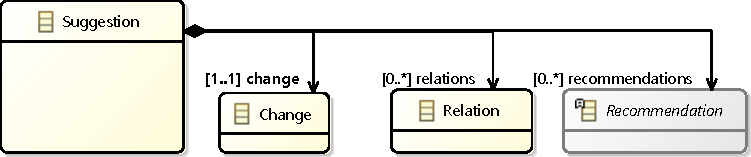
\includegraphics[width=\columnwidth]{images/Suggestion.pdf}
    \caption{A \textsf{Suggestion} holds for a single \textsf{Change} linked to 
		elements in a View Type through \textsf{Relation}s, and consists of a set of \textsf{Recommendation}s.}
    \label{fig:Suggestion}
\end{figure}

A \textsf{Change} refers to an \textsf{Operator} that may be parameterised with 
extra data, and contains contextual information (in \textsf{ApplicationPattern}). 
Change \textsf{Operator}s may target \emph{any} instanciable metamodel element, 
thus referring to the class \textsf{NamedElement} in \textsc{Mof}. Note that we 
will distinguish between \emph{primitive} and \emph{complex} \textsf{Operator}s,
depending on the number of such \metamodel elements an \textsf{Operator} acts on.

Since \viewtypes are structurally \metamodels, we reviewed the literature to
identify relevant change \textsf{Operator}s. The change catalogue proposed by 
\cite{herrmannsdoerfer_extensive_2011} presents 27 \emph{primitive}, and 34
\emph{complex} operators. We integrated all primitive, and 7 complex operators
in our work, which were selected because they constitute 72\% of all complex
changes appearing in a large case study (cf. \cite{khelladi_detecting_2015}). 

\textsf{Operator}s are enriched with a \emph{severity}: \emph{Major}
(abbreviated as \textsf{M}), \emph{miNor} (\textsf{N}) and \emph{Ignore} 
(\textsf{I}). 
When applied to a \metamodel, the \textsf{Operator}s in \textsf{I} have no effect
on the corresponding \viewtypes; \textsf{Operator}s that can break the relationship
between \textsf{MM }and its \viewtypes are categorised as \textsf{M}; the rest of the
\textsf{Operator}s are \textsf{N}, since they are not breaking and can enrich 
the \viewtypes with additional information.

\begin{figure}[t]
    \centering
    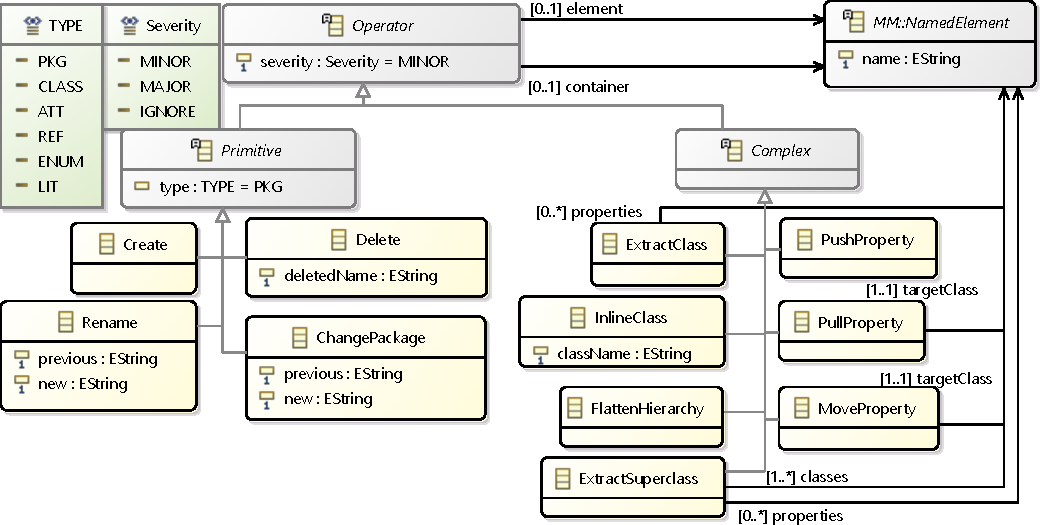
\includegraphics[width=\columnwidth]{Change.pdf}
    \caption{Possible \textsf{Operator}s for \metamodel evolution.}
    \label{fig:Change}
\end{figure}

The evolution steps of Figure \ref{fig:FSM} make use of different \textsf{Operator}s.
\begin{itemize}
	\item In Step 1 (depicted from Figure \ref{fig:FSM:Init} to \ref{fig:FSM:Relevant}),
	the following sequence of \textsf{Operator}s is applied:
	$$\langle \mathsf{PushProperty} \cdot \mathsf{Rename} \cdot \mathsf{Rename} \rangle$$
	First, \textsf{PushProperty} pushes down $\mathsf{Named} \squaredots \mathsf{name}$
	(i.e. pushes down the \textsf{element} \textsf{name} in the \textsf{container}
	\textsf{Named})
	into each subclass (namely, \textsf{FSM}, \textsf{State} and \textsf{Transition});
	then \textsf{Rename} is applied to the \textsf{element} \textsf{name}, 
	located respectively in \textsf{container}s $\mathsf{FSM}$ and 
	$\mathsf{Transition}$, thus obtaining the result of Figure \ref{fig:FSM:Relevant}.
	
	\item Step 2 only consists of the following \textsf{Operator}s sequence:
	$$\langle \mathsf{Create} \cdot \mathsf{Create} \cdot \mathsf{Create} \rangle$$
	where each \textsf{Operator} adds a new Attribute \textsf{element} in 
	\textsf{container} \textsf{Transition}, ending up in the situation of
	Figure \ref{fig:FSM:Guard}.
	
	\item Step 3 requires a longer sequence of \textsf{Operator}s, since it creates
	a new class hieararchy under \textsf{Expression}. However, this sequence may
	start with the following:
	$$\langle \mathsf{Delete}^3 \cdot \mathsf{Create}^2 \cdot \ldots \rangle$$
	The three first \textsf{Delete} undo the \textsf{Create} operations of Step 2
	(thus, referring to the same \textsf{element}s and \textsf{container}); and
	the two following \textsf{Create} create the new \textsf{Expression} class
	(with the default package as a \textsf{container}) and the \textsf{guard}
	reference (with \textsf{Transition} as a \textsf{container}).
\end{itemize}
With these examples, we immediately notice that some \textsf{Operator}s
in a \textsf{Change} sequence may depend on previous ones (e.g. \textsf{Rename}
in Step 1 should only be performed after \textsf{PushProperty}); while others
may freely commute (e.g. the \textsf{Create} in Step 2 may be performed in any 
order).
\subsection{Relation}
\label{sec:Suggestion:Relation}

The \textsf{Relation} part provides traceability links between \textsf{MM}
all the corresponding \textsf{changed} and \textsf{impacted} elements.
% elements that are \textsf{changed}, and all \viewtype elements that are 
% \textsf{impacted} by that change. 
One \textsf{MM} element change
may impact several elements in the same \viewtype, but may also potentially
impact several \viewtypes. We only require so-called \emph{links}; however richer
data structures for traceability may be used \cite{Batot-Cabot-Gerard:2021}.

The way these traceability links are computed are left as implementation
details, and may happen in two ways: \emph{on-the-fly} whenever an \textsf{MM} element is evolved; and \emph{offline}
after a complete evolution session has terminated---either based on diffing \cite{Kehrer-Kelter-Taentzer:2011}, or using 
operation-based approaches \cite{J:Lippe-Oosterom:1992}.

\begin{figure}[t]
    \centering
    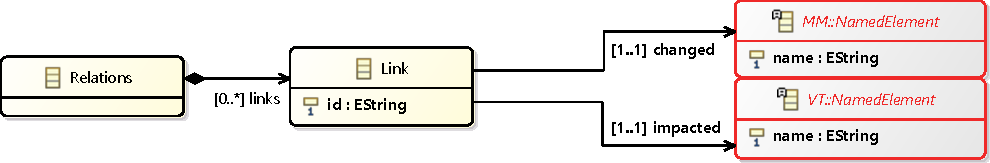
\includegraphics[width=\columnwidth]{Relation.pdf}
    \caption{\textsf{Relation}s between \textsf{MM} elements and \textsf{VT} elements.}
    \label{fig:Relation}
\end{figure}

In the \textsf{FSM} example associated to the initial \textsf{VT\_FSM} of \cref{fig:VT:VMM},
we would have, among others, the following relations (with \textsf{Link}s denoted 
as e.g.~$\mathsf{<} \mathsf{changed} ; \mathsf{impacted} \mathsf{>}$):
\begin{itemize}
	\item Since computing the \textsf{name}s in \textsf{VT\_FSM} requires access
	to $\mathsf{Named \squaredots name}$, the following \textsf{Link}s would be
	created: 
	$\mathsf{<} \mathsf{Named \squaredots name} ; \mathsf{VT\_FSM \squaredots name} \mathsf{>}$;
	$\mathsf{<} \mathsf{Named \squaredots name} ; \mathsf{State \squaredots name} \mathsf{>}$;
	$\mathsf{<} \mathsf{Named \squaredots name} ; \mathsf{Transition \squaredots name} \mathsf{>}$.

	\item Creating an instance of \textsf{State} requires to take into account
	the value of $\mathsf{State \squaredots kind}$, which would produce the following
	\textsf{Link}s: 
	$\mathsf{<} \mathsf{State \squaredots kind} ; \mathsf{State} \mathsf{>}$;
	$\mathsf{<} \mathsf{State \squaredots kind} ; \mathsf{Initial} \mathsf{>}$;
	$\mathsf{<} \mathsf{State \squaredots kind} ; \mathsf{Regular} \mathsf{>}$.
	Depending on the precision of the traceability analysis, the following may
	eventually be produced as well: 
	$\mathsf{<} \mathsf{Kind \squaredots REGULAR} ; \mathsf{Regular} \mathsf{>}$ and
	$\mathsf{<} \mathsf{Kind \squaredots INITIAL} ; \mathsf{Initial} \mathsf{>}$.
	%\LC{Again, for FINAL too?}\MA{The \textsf{Link}s are established on the initial version, \emph{\textbf{before} the evolution step. 
	%The next bullet (``After Step 2''!!!) explicitly says what you want to put here, which is a wrong place to do so.}}
	


	\item After Step 2, some \textsf{Link}s between the newly added attributes
	in $\mathsf{FSM \squaredots Transition}$ and the corresponding attributes in 
	$\mathsf{VT\_FSM \squaredots Transition}$ may be added as well. New 
	\textsf{Link}s taking into account the newly added literal in \textsf{Kind}
	would be added, similarly to the previous point.
\end{itemize}
\subsection{Recommendation}
\label{sec:Suggestion:Recommendation}

While a \textsf{Change} concerns \textsf{MM}, a \textsf{Recommendation} describes
an \textsf{Action} a methodologist may perform on \textsf{VT}. In our approach, we
issue a \textsf{Recommendation} for each \viewtype element impacted by a 
\textsf{Change}. We identified four kinds of \textsf{Action}s: a \textsf{REM}ove
\textsf{Action} indicates that a \viewtype element is no longer associated to an
\textsf{MM} element; an \textsf{ADD} suggests that a representation for a newly 
created \textsf{MM} element should be added in a \viewtype; an \textsf{UP}date
\textsf{Action} suggests to update a 


\begin{figure}[t]
    \centering
    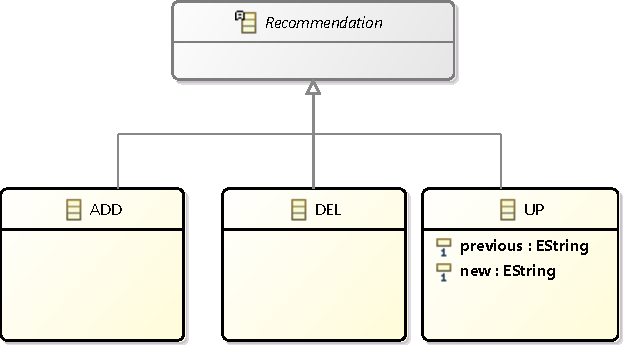
\includegraphics[width=0.8\columnwidth]{Recommendation.pdf}
    \caption{\textsf{Recommendation}s suggested after a \textsf{Change}}
    \label{fig:Change}
\end{figure}


\section{Approach} 
\label{sec:Approach}

For the \metamodel-\viewtype co-evolution we identified 34 operators from the change catalogue proposed by \cite{herrmannsdoerfer_extensive_2011}, which contains 27 \textit{primitive} and 34 \textit{complex} operators. Our work addresses all primitive and 7 complex operators. We choose the complex operators based on the work of \cite{khelladi_detecting_2015} who claims that these changes constitute 72\% of all complex changes during the evolution of GMF. \Cref{tab:suggestions} summarises the operators, their types, corresponding suggestions, and severity of applying these operators. We divided the chosen operators into three severity categories: major (M), minor (N), and ignore (I).
\MA{IMO, it's not the severity that "divides" the operators. 
The severity "characterises", or "classifies". However, I suggest to 
use some kind of classification of operators to avoid the long list.
cf. Herrmannsdoerfer et al. among others.}
When applied to a \metamodel, the operators in the latter category have no effect on the corresponding \viewtypes. The operators that can break the relationship between the evolving \metamodel and the corresponding \viewtypes are categorised as major. We classify the rest of the operators as minor since they are not breaking and can enrich the \viewtypes with additional information.

Among the primitive operations the creation of various entities are of minor severity as they do not influence the existing relation between the \metamodel and corresponding \viewtypes. For the creation of package, class, data type, and enumeration, we only notify the modeller about the addition of these entities. 
According to the \metamodeling formalism proposed by \cite{herrmannsdoerfer_extensive_2011}, attributes and references, and literals, have composition relation with resp. classes and enumerations. Therefore, in the event of the creation of these entities, we first identify the \viewtypes that reference the corresponding container (i.e., class or enumeration) and suggest the addition of the new entities for these \viewtypes.

The deletion of a package is possible iff it is empty and therefore, this operation can be safely ignored. Deleting class, feature, data type, and enumeration can have major consequence if these entities are referred from one or more related \viewtypes as the partial representation relation with the corresponding \metamodel no longer holds. Therefore, the suggestion is to remove these entities also from the \viewtypes.

The \textit{Make Class Abstract} and \textit{Drop Class Abstract} are about making an existing class abstract and vice versa. As these operations only changes the abstraction without modifying the list of features, they can be ignored in the context of \viewtype co-evolution. 

The deletion of an opposite reference removes access to the referenced entity from the referencing one. The corresponding suggestion is to remove the references also from the \viewtype. \textit{Merge Literal} removes a literal and replaces its occurrence with another one. Therefore, applying this operations triggers the suggestion to replace the deleted literal with an existing one in the \viewtype. \textit{Rename} and \textit{Change Package} operators generate suggestions to do the same (i.e., renaming and changing package location) on the related \viewtypes.

The \textit{Add Super Type} and \textit{Remove Super Type} operators adds and removes inherited features from an existing class. Accordingly, the corresponding suggestion suggests the addition or removal of inherited features wherever the child class is referenced in the \viewtype. Although the suggestion for the former is of minor severity, the removal of features can break the \viewtype and hence, is classified as major.

The \textit{Make Attribute Identified} and \textit{Drop Attribute Identifier} operators adds or removes a constraint that ensures the uniqueness of the attribute values. The \textit{Make Reference Composite} and \textit{Drop Reference Composite} adds or removes the containment restriction for an reference. Since, these are instance level constraints, they do not influence the \viewtype and therefore, can be ignored.

\HM{Discuss \textit{Make ref opposite and drop ref opposite}}

The \textit{Move Property} operator triggers the suggestion to update the corresponding location in the \viewtype. Pushing a property down in the hierarchy removes the property from the super class and therefore, it needs to be removed from the \viewtype wherever it is referred using a reference of the super class. The \textit{Pull Up} operator can be applied iff the corresponding feature is present in all the child classes. Since the feature is still accessible via inheritance, this does not trigger any suggestion for the related \viewtypes.

Extracting super class does not influence the effective set of features and therefore, triggers a minor suggestion for replacing some occurrences of the child class reference with the parent. The \textit{Flatten Hierarchy} moves all the features from the parent to the child classes and deletes the parent class. Therefore, this triggers a major suggestion for replacing all the references of the removed super class with the appropriate child class reference. Since the effective features of the child classes remain the same before and after fattening, we offer no suggestion for the child classes. The \textit{Extract Class} operator groups a set of features into a new delegate class and replaces their occurrences with a reference to the delegate class. The \textit{Inline Class} operator is the exact opposite of \textit{Extract Class}. Both triggers a major suggestion of adapting the location of any related feature referenced in the \viewtype.

\begin{table*}[ht!]
\caption{Suggestions per change operator. The Primitive and Complex operators are denoted respectively with P and C. \MA{Give a legend for the abbreviations in "Type" and "Severity" columns. Similarly, the "TYPE" values are never explained in the text (and should be part of the legend as well).}} \label{tab:suggestions}
\centering
\begin{tabular}{|l|c|p{.33\linewidth}|p{.31\linewidth}|c|}
\hline
Operator & Type & Condition to offer suggestion & Suggestion & Severity \\ \hline \hline

Create Package &  
\multirow{4}{*}{P} & 
\multirow{4}{*}{None} &      
\multirow{4}{*}{Notify the addition of the new entities} &
\multirow{4}{*}{N} \\ \cline{1-1}
Create Class &  &    &      &             \\ \cline{1-1}
Create Data Type &  &    &      &             \\ \cline{1-1}
Create Enum &    &  &      &             \\ \hline

Create Reference & \multirow{4}{*}{P} &    
\multirow{4}{*}{\parbox{\linewidth}{Containers (i.e., package, class) to which the entity is added are referenced from the \viewtype}} &      
\multirow{4}{*}{\parbox{\linewidth}{Suggest the addition of the new entities in the \viewtype}} &
\multirow{4}{*}{N} \\ \cline{1-1}
Create Opposite Ref. &   &   &      &             \\ \cline{1-1}
Create Attribute &  &    &      &             \\ \cline{1-1}
Create Literal &    &  &      &             \\ \hline

Delete Package  & P &
None & None. & N \\ \hline

Delete Class & \multirow{4}{*}{P} & 
\multirow{4}{*}{\parbox{\linewidth}{Entity or corresponding feature referenced by \viewtype}} &
\multirow{4}{*}{Suggest the deletion of the corresponding entity} & \multirow{4}{*}{M}           \\ \cline{1-1}
Delete Feature  &     & &      &             \\ \cline{1-1}
Delete Data Type  &    &  &      &             \\ \cline{1-1}
Delete Enum  &   &   &      &             \\ \hline

Make Class Abstract  & \multirow{2}{*}{P} & \multirow{2}{*}{None}     & \multirow{2}{*}{None}     & \multirow{2}{*}{I} \\ \cline{1-1}
Drop Class Abstract  &  & &  & \\ \hline

Delete Opposite Ref.  & P &  \Viewtype refers the referencing class & Suggest referenced class and corresponding features not accessible & M            \\ \hline
Merge Literal  & P&  Merged literal referenced by \viewtype    & Suggest the replacing literal  & M            \\ \hline
Rename  & P& Old name referred in the \viewtype  &  Suggest the old name and the corresponding new name  & M \\ \hline
Change Package  & P& Corresponding entity referred in \viewtype & Suggest changing of the package & M \\ \hline
Add Super Type  & P& Child types are referred in \viewtype & Suggest addition of inherited features for all child types & N  
% (does ST has property?) yes.       
\\ \hline
Remove Super Type  & P& Features inherited from removed super type are referred in \viewtype & Suggest removal of features that were previously inherited & M 
% (super type is empty?) no.     
\\ \hline
Make Attr. Identifier   & \multirow{4}{*}{P} &  \multirow{4}{*}{None}    &  \multirow{4}{*}{None}    & \multirow{4}{*}{I}            \\ \cline{1-1}
Drop Attr. Identifier  & &      &      &     \\ \cline{1-1}
Make Ref. Composite  & &      &      &             \\ \cline{1-1}
Switch Ref. Composite  & &      &      &             \\ \hline
Make Ref. Opposite  & P&      &   Discuss   &             \\ \hline
Drop Ref. Opposite  & P&      &    Discuss  &             \\ \hline
Move Property  & C &  Corresponding property referred in \viewtype  & Suggest the source and destination of the moved property & M \\ \hline
Push Property   & C & Super class referred in \viewtype  & Suggest removal of features from super class & M \\ \hline
Pull Property   & C & None & None & I \\ \hline
Extract Super Class  & C & Child classes referred in \viewtype  & Suggest possible replacement of child classes with newly created super class & N  \\ \hline
Flatten Hierarchy   & C & Removed super class is referenced in \viewtype &   Suggest removal of super class and replace all of its occurrences with appropriate child class   &  M           \\ \hline
Extract Class   & C & Extracted features from the delegate class are referred in \viewtype & Suggest the moving of features to the delegate class from the original class & M \\ \hline
Inline Class   & C & Delegate class is referenced in \viewtype & Suggest moving of features from delegate class to class that referenced the delegate class & M            \\ \hline

\end{tabular}
\end{table*}
\section{Formalization}
\label{sec:Formalization}
In this chapter we define the terms suggestion and applicable suggestion. We introduce possible ways to refine a suggestion and to add domain specific knowledge.

\begin{figure}
    \centering
    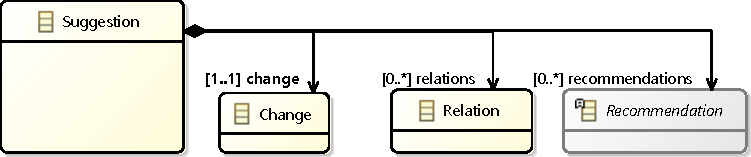
\includegraphics[width=\columnwidth]{images/Suggestion.pdf}
    \caption{A \textsf{Suggestion} holds for a single \textsf{Change} linked to elements in a View Type through \textsf{Relation}s, and consists of a set of \textsf{Recommendation}s.}
    \label{fig:Suggestion}
\end{figure}

\begin{figure}
    \centering
    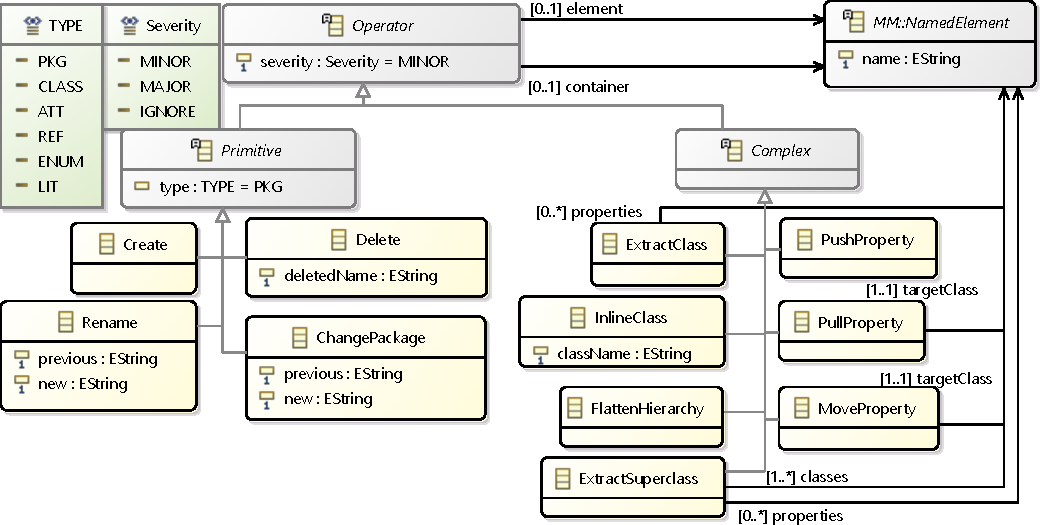
\includegraphics[width=\columnwidth]{Change.pdf}
    \caption{Possible \textsf{Change}s operated on a \metamodel \MA{This really corresponds to the \textsf{Opeartor} column of Table \ref{tab:suggestions}, where \textsf{ApplicationPattern} maps the column \textsf{Condition to offer...}.}}
    \label{fig:Change}
\end{figure}


\begin{definition}[Suggestion]\label{def:suggestion}
We define a suggestion $SUG$ as a 4-Tuple of a type of a change on the \metamodel $MMC$, a view generation transformation $VGT$ (which link to the \metamodel and the \viewtype),  constraints $CON$ and a suggestion content $SUC$. Short: $SUG = (MMC, VGT, CON, SUC)$
\end{definition}
Possible $MMC$ are defined in \cref{tab:suggestions}. A suggestion always contains one change. Change sequences that have domain semantics should define a new complex change, because the contained domain knowledge is interesting for other analyses besides suggestions. The view generation operators $VGO$ are defined in \cref{fig:model-query-operators}. They can be combined to a $VGT$. $VGTs$ may form a hierarchy that can be used for the refinement of suggestions. The constraints are defined on either the \metamodel, its instance, the view generation operators or the target \metamodel. Constraints may also form a hierarchy for the refinement of suggestions. The $SUC$ is either a textual description of the suggestion or a formalisation of possible changes or a change on the \viewtype or a combination of all three. Either the textual description or the formalisation and the possible changes are preferable as it enables the methodologist to precisely define the change on the \viewtype \metamodel as well as giving some rationale. The formalization represents the middle way between the directly applicable definition of the changes and the textual description.

An example for a suggestion is \textit{(Create Attribute in metamodel, Select,  "viewtype is identity mapping of metamodel", ("As the viewtype is an identity mapping of the underlying metamodel, we suggest to update the viewtype to also include the new attribute.", Create Attribute in viewtype metamodel))}. A possible refinement could also include the $CON$ \textit{attribute is marked as hidden} which may semantically take precedence over the identity mapping and the suggestion contains the $SUC$ \textit{"As the attribute is marked as hidden, we suggest to not update the viewtype."}. Both $VGT$ and $CON$ enable the methodologist to include semantic domain specific knowledge into the suggestions.

\HM{I have a slightly detailed version of the formalism. Majority of the concepts are similar to \Cref{def:suggestion} with some added details which should allow connecting \Cref{tab:suggestions}.}
\MA{Oh... I didn't see that before! This somehow matches Figs. \ref{fig:Change} and \ref{fig:Suggestion}, modulo the details of where things are placed in the structure (tuple in math formalisation vs. elements of the MM). But they are similar in essence!}

\begin{definition} [\Metamodel change]
    We define a \metamodel change ($MMC$) as a 3-element tuple: $MMC = (OP, E, NE)$ where $OP$ is a \metamodel change operator, $E$ is a set of entities from the \metamodel, which the $OP$ is applied to, and $NE$ is the set of entities that are affected by the application of $OP$.
\end{definition}
The $OP$s we address are listed in \Cref{tab:suggestions}. The entity sets $E$ and $NE$ can be empty in certain cases. For example, the creation of an element does not affect any existing entity but creates one or more. Therefore, in this case $E$ is an empty set and $NE$ contains the newly created entities.

\begin{definition} [\Viewtype evolution]
    \Viewtype evolution is a set of 3 mapping functions: $VTE$ = \{$AD$, $RM$, $MV$\}. Each of these functions encapsulates the creation, deletion, and moving operations that are applied on \viewtype ($VT$) and/or view generation transformation ($VGT$). We further define these functions as follows: $AD$ : ($D$, $NE$) $\rightarrow$ $ND$, $RM$ : ($D$, $E$) $\rightarrow$ $D$, and $MV$ : ($D$, $E$, $NE$) $\rightarrow$ $ND$. Here $D$ is the $VT$ and/or $VGT$ and $ND$ is the transformed state of the corresponding entities. 
\end{definition}

\begin{definition}[Suggestion (v2)]
    We define a suggestion as a 5-tuple of a type of a change on the $MMC$ and has the form $SUG$ = ($MMC$, $VTE$, $EVM$, $CON$, $SUC$), where 
\end{definition}

\section{Evaluation}
\label{sec:Evaluation}


\textbf{Limitations:}
\begin{itemize}
    \item we do not support \metamodel \metamodel co-evolution [we’re looking at view-based only, not necessarily V-SUM, so MM-MM co-evolution not a concern]
    \item we do not support \metamodel model co-evolution
    \item \st{we only support co-evolution from the metamodel to the viewtype (which is actually not a limitation, since conceptually one can still start at the viewtype)}
    \item \st{we only support one metamodel as the source of a viewtype}
\end{itemize}
\section{Related Work}
\label{sec:RW}

\begin{itemize}
    \item \metamodel version co-existence (Alexander Egyed)
    \item MM to MM co-evolution
    \item database view co-evolution
\end{itemize}

\section{Conclusion}
\label{sec:Conclusion}

conclusion and future work \cite{braun_classification_2014}


\LC{TODO: probably future work: talk about (i) more complex patterns to give better suggestions;
(ii) domain-specific approach / refinements to approach, with illustration on
state charts?}
\TW{I added an example in \cref{sec:Conditions}}

discuss work, limitations, where it should go

\st{viewtype transformations}


Future work - make suggestions applicable 

\begin{comment}
\TW{TODO: remove the formalisation, cut the definition short and try to define the idea more precisely} \begin{definition}[Applicable Suggestion]
We define an applicable suggestion as a 3-Tuple of a suggestion, a transformation of the $VGT$($TVGT$) and a transformation between the $MMC$ and the $SUC$($TSUC$). Short $ASU = (SUG, TVGT, TSUC)$
\end{definition}
\HM{This definition seems unclear to me. I am also not sure of its relevance in the context of this work.} \TW{As discussed in the meeting, this definition is not part of the scope of this paper but future work on how to use our definitions. We may keep it as limitation or move its content to the future work section (a formal definition won't make sense there, but i think we should keep the ideas and present them.)}
Note that the $SUC$ of an $ASU$ has to contain the definition of the change on the \viewtype \metamodel. The $TVGT$ transforms the $VGO$, e.g. by adding a newly created attribute as input. The $TSUC$ transforms the change on the \metamodel in a change on the \viewtype \metamodel. In the example above, the change on the \metamodel will be transformed by changing its target from the \metamodel to the \viewtype \metamodel. A suggestion can have multiple applicable suggestions from which the methodologist can chose the most appropriate one.
\end{comment}


% \bibliographystyle{IEEEtran}
\printbibliography
\end{document}
